\section{Results}
\label{sec:experiments}

%\mb{I find ``\emph{around-right}'' more informative as a name than
%  ``\emph{template}''. I am replacing it in the text, but it should
%  also be updated in the figures.}

% We conducted three different experiments where we evaluated the accuracy of the models in terms of how many test commands were exactly translated
% into corresponding test actions. 
% \citet{Lake:Baroni:2017} found that RNNs models are achieve nearly perfect performance when tested on a random split of SCAN but accuracy drops significantly
% (down to around 20\% for their best performing model) when the network is tested on composing new meanings after being exposed only to shorter samples.

% In order to make our results comparable with previous work on SCAN each training set consists of 100,000 examples sampled with replacement
% from each related train/test split. We decided to replicate experiment 1 of \cite{Lake:Baroni:2017} that simply uses a random split
% of the SCAN dataset divided into a train (80\%) and test (20\%) set. This would act as a first comparison with the RNNs results reported in their work.

% \subsection{Experiment 1: random split and primitive generalization}
% \label{subsec:exp1}

%\subsection{General results}

%\mb{Please add table with our results for the 3 splits for both the
%  best-overall and the split-best settings (and sds), as well as the
%  L\&B, Loula et al and Bastings et al results (for the latter, the
%  GRU+att 12.5 jump result should suffice.}


\begin{table}[tb]
  \begin{footnotesize}
    \begin{center}
        \scalebox{0.96}{
          % \begin{tabular}{l | p{2cm} | p{2cm} | p{2cm}}
          \begin{tabular}{l | r | r | r}
             & \textbf{random} & \textbf{jump} & \textbf{around-right} \\ \hline
             LSTM & 99.8 & 1.2 & 2.5$\pm$2.7 \\
             GRU & \textbf{100.0}$\pm$0.0 & 12.5$\pm$6.6 & --  \\
             \hline
             CNN & 100.0$\pm$0.0 & \textbf{69.2}$\pm$8.2 & \textbf{56.7}$\pm$10.2 \\
        \end{tabular} 
    }
    \end{center}
  \end{footnotesize}
  \caption{Test accuracy (\%) on SCAN splits (means across 5 seeds,
    with standard deviation if available). Top LSTM results from
    \newcite{Lake:Baroni:2017}/\newcite{Loula:etal:2018}, GRU from
      \newcite{Bastings:etal:2018}.}
\label{table:main_results} 
\end{table}

Our main results are in Table \ref{table:main_results}. Like the
RNNs studied by \newcite{Lake:Baroni:2017}, our CNN has no problem in
the \emph{random} split. However, its results are much higher than
those of the best RNNs in the challenging \emph{jump} and
\emph{around-right} splits. Still, their performance is far from perfect.

The SCAN tasks are designed to be easy for a system that has learned
the right composition rules. Perhaps, CNNs do not achieve 100\%
accuracy because they only learned a subset of the necessary
rules. For example, they might correctly interpret the new
expression \emph{jump twice} because they induced a \emph{X twice}
rule at training time, but fail at \emph{jump
  thrice} because they missed the corresponding \emph{X
  thrice} rule. Since SCAN semantic composition rules are associated
with single words in input commands, we can check this hypothesis by
looking at error distribution across input words. It turns out instead that,
% in neither the \emph{jump} nor the \emph{around-split},
errors are not associated to specific input commands.  Figure
\ref{fig:error_distributions} shows error proportions across input
words (over total occurrences of the words) for the best models in
each split. We observe a relatively stable proportion of errors across
command words. Direct inspection reveals no traces of
systematicity, either. Indeed, we often find minimal pairs in which changing
one action verb with another (distributionally equivalent in SCAN)
turns a correctly executed command into a failed one. For
example, in the \emph{jump} split, the CNN correctly executes
``\emph{jump left after walk},'' but fails ``\emph{jump left after
  run}'' (jumping is forgotten). Analogously, in the
\emph{around-right} split, ``\emph{run around right}'' is correctly
executed, but ``\emph{walk around right}'' isn't (the CNN stops too
soon).

\begin{figure}[tb]
    \centering
    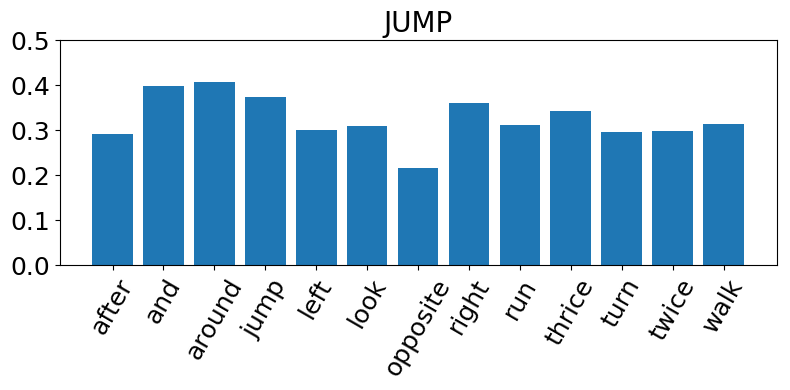
\includegraphics[width=.4\textwidth,keepaspectratio]{figures/jump_error_dist.png}
    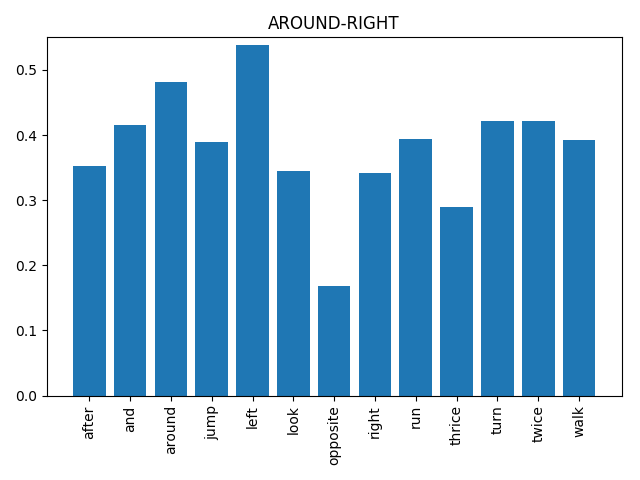
\includegraphics[width=.4\textwidth,keepaspectratio]{figures/template_error_dist.png}
    \caption{Proportion of commands with a certain command word (over word
      total) wrongly executed by best CNNs of
       \emph{jump} and \emph{around-right} splits.}
    \label{fig:error_distributions}
\end{figure}

\paragraph{Robustness} Fig.~\ref{fig:exp1} shows a big difference in
stability between \emph{random} and the other splits across top
hyperparameter configurations. The \emph{random} results are very
stable. \emph{Jump} accuracy is relatively stable across
hyperparameters, but has large variance across initialization
seeds. For the most challenging \emph{around-right} split, we observe
instability both across seeds and hyperparameters (although even the
lowest end of the reported accuracies is well above best RNN
performance in the corresponding experiments). Another question is
whether the best configurations are shared, or each split requires an
ad-hoc hyperparameter setting. We find that there are configurations
that achieve good performance across the splits. In particular, the
\emph{best overall configuration}, found by minimizing ranks across
splits, has 0.01 learning rate, 25-tokens batch size, 0.25
dropout, 6 layers, 512 layer dimensionality, and kernels of width
5. Such model was 13th best (of about 2.5K explored) on the
\emph{random} split (with mean cross-seed accuracy of 99.92\%, off
by 0.05\% from top configuration), 32th on the \emph{jump} split
(60.67\% mean accuracy, off by 8.62\%), and 2nd in the
\emph{around-right} split (mean 53.25\% accuracy, off by 3.45\%).
% \rd{from here} We found the best overall model by first selecting only
% the models that ranked 300th or higher in all three splits. Then for
% every model we selected the lowest rank (low-rank) among the three
% split and we picked as best overall the model with the highest
% low-rank. As an example, if only two models were among the top 300 on
% all three splits and model \textit{A} was ranked 1st, 2nd and 50th on
% random, jump and around-right respectively, and model \textit{B}
% ranked 45th, 10th and 10th then model \textit{A} would have a low-rank
% value of 50 and model \textit{B} a low-rank value of 45. Model B would
% then be selected as best overall model.

% \mb{Should we say how the best overall was found?} \rd{to here. Does it make sense?}
% Experiment 2 and 3 in section \ref{subsec:exp2} and \ref{subsec:exp3} used the aforementioned model.

% After a preliminary experiment we found a subset of parameters showing reasonable performance and conduceted a large hyperparameters
% search on every split.
% We varied batch sizes (in term of number of tokens in the batch: 25, 50, 100, 200, 500 and 100), learning rates
% 0.1, 0.01, 0.001), the embedding dimensions (128, 256, 512), amount of dropout used (0, 0.25, 0.5) \cite{srivastava:eta:2014}, number of convolutional
% layers for both the encoder and decoder (6, 7, 8, 9, 10) and width of the convolutional kernel (3, 4, 5).
% We then cross validated the top-300 models across 5 different runs. Accuracy and standard deviation are presented in figure \ref{fig:exp1}. 
% We inspected the average accuracy of the model note that the amount of standard deviation of the top-300 models reached a performance range with a lower limit that was always
% considerably lower than the best model for each split, making us think that considering the top-300 models was
% a right choice that included tha real best model for every split. In other words, the accuracy for the best model and the 300th one formed a large range.
% \footnote{This might not seem the case for the results on the random split where the range is (95.17, 99.97). However the standard deviation across all 300 models does not
% exceed 2.7}
% When analyzing the the resulting models for every split we computed a \textbf{best overall model} across all splits which
% was a model trained with a learning rate of 0.01, a 25 tokens per batch, dropout applied with probability 0.25, it had 6 layers in both the encoder and the decoder,
% embedding dimension of 512, a convolutional kernel of width 5. Such model was ranked 13th on the random split (with an accuracy of 99.92\% off by 0.05\%), 
% 32th on the jump split (60.67\% accuracy, off by 8.62\% compared to the top performing model for the split),
% and 2nd in the template split (53.25\% accuracy, off by 3.45\%)
% Experiment 2 and 3 in section \ref{subsec:exp2} and \ref{subsec:exp3} used the aforementioned model.

\begin{figure}[tb]
    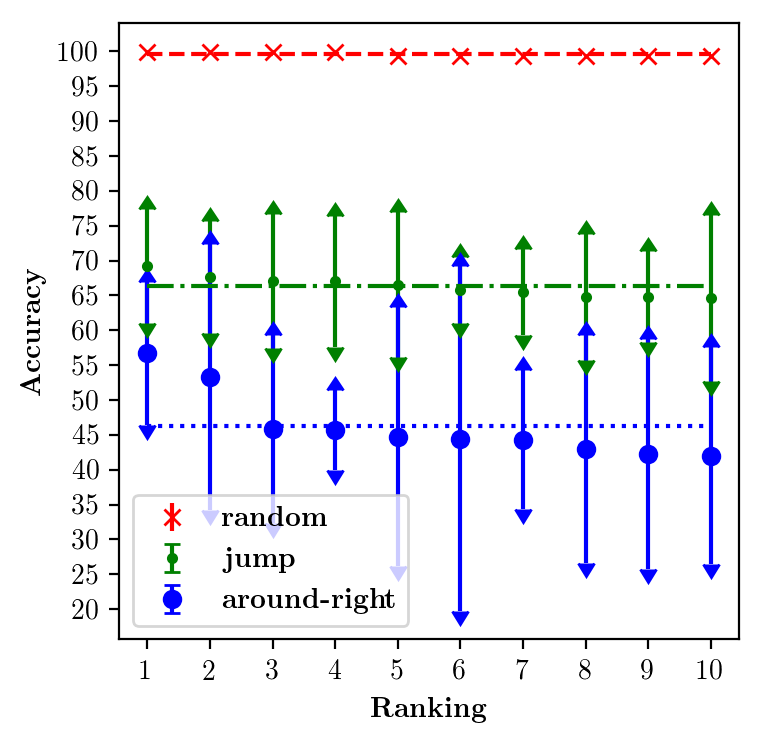
\includegraphics[width=.4\textwidth,keepaspectratio]{figures/accuracies_all_splits.png}
    \centering
    \caption{Accuracies (\%) of top-10 models on \emph{random}, \emph{jump} and \emph{around-right}. Arrows
      denote standard deviations, dashed lines average accuracy across top-10.
      % \mb{means across what? Also, it would be better if
      %legend order was random/jump/around-right}
      }
    \label{fig:exp1}
\end{figure}

\paragraph{Impact of kernel width}
\label{subsec:exp2}

One important difference between recurrent and a convolutional
architectures is that in the former it is left to the learned dynamics
of the recurrent matrix to determine context size, whereas the kernel
width of a CNN imposes a strong prior on the window of elements to be
processed together. We conjecture that relatively wide encoder and
decoder widths, by naturally pushing the network to keep wider
contexts into account, might favour the acquisition of template-based
generalizations, and hence better compositionality. To investigate
this, we varied encoder and decoder widths of the best-overall model
between 1 and 5.\footnote{At least on the encoder side, larger widths
  seem excessive, as the longest commands are 9-word-long.}

% We consider the use of convolutional filters as an interesting dimension to inspect, especially when considering 
% its ability to possibly assess the small and self contained semantics of single words within the larger context of a sentence \rd{\dots make a proper example with SCAN]}.
% The desired systematic compositionality that we seek to find in modern neural networks could indeed be described as the
% human ability to extract, process and combine small unit that are semantically meaningful, in order to create a larger and again meaningful semantic block.
% The hypothesis of the use of convolutions as an important parameter for the ability of the network
% to correctly process semantic compositionality is investigated in our second experiment presented in section \ref{subsec:exp2}.

\begin{figure*}[tb]
    \centering
    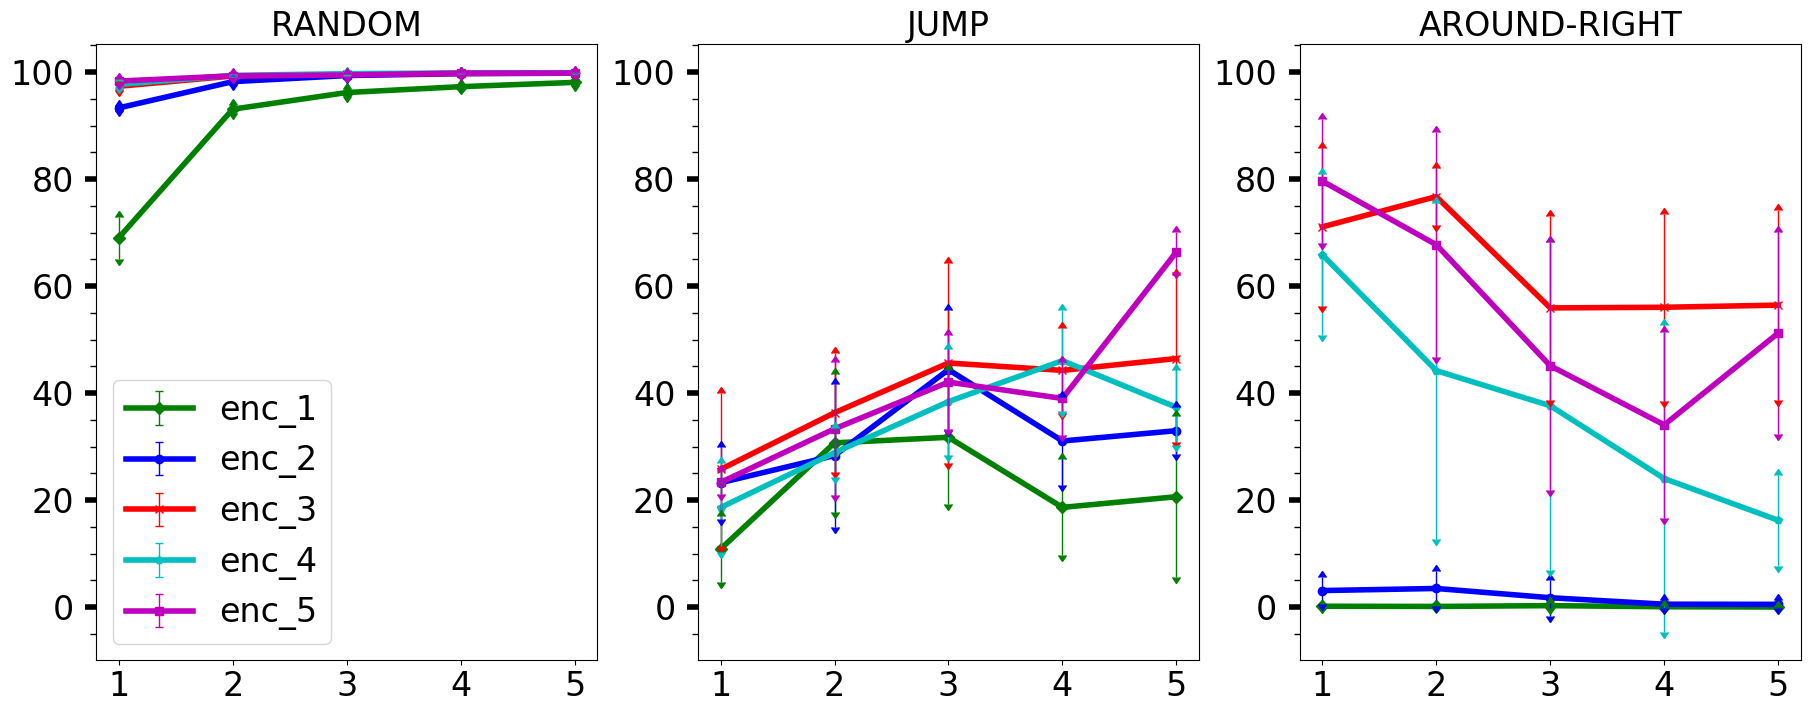
\includegraphics[width=\textwidth,keepaspectratio]{figures/kernel_exp.png}
    \caption{Mean accuracies (\%) across 5 seeds, in function of decoder (x axis) and encoder (colors) kernel widths. Arrows denote standard deviations.
    %More natural order would be random/jump/around-right.
%    \mb{Also crop actual file and enlarge figure.}
    }
    \label{fig:kernel_exp}
\end{figure*}

As shown in Fig.~\ref{fig:kernel_exp}, the \emph{random} split confirm
our expectations, as both wider encoder and decoder windows improve
performance. The \emph{jump} results follow the same trend, although
in a less clear-cut way. Still, the narrowest encoder-decoder
combination shows the worst performance, and the widest one the top
one. For the \emph{around-right} split, it's also better to use the
widest encoder, but top performance is achieved with the
\emph{narrowest} decoder (width$=$1). Indeed, with the narrow decoder
we obtain \emph{around-right} accuracies that are even above the
absolute-best \emph{jump}-split performance. Since the novel output
templates in the \emph{around-right} split are by construction long
(they involve executing an \emph{around} command that involves
repeating an action 4 times), we would have rather expected models
keeping track of a larger decoding window to fare better particularly
in this case. We tried to gain some insight on the attested behaviour
by looking at performance distribution in function of input and output
length, failing to detect different patterns in the wide-decoder
\emph{jump} model vs.~the narrow-decoder \emph{around-right} model
(analysis not reported here for space reasons). Looking qualitatively
at the errors, we note that, for both splits, the narrower decoder
tends to skip trajectory sub-chunks (e.g., executing ``\emph{jump around
right}'' with 3 instead of 4 right turns followed by jumps), whereas
the wider kernel is more likely to substitute actions (e.g., turning
left instead of right) than undershooting the length. This
impressionistic observation is supported by the fact that, for both
splits, the narrow-kernel errors have considerably larger variance
with respect to ground-truth length. These analyses, however, only confirm our
initial conjecture that a wider decoder kernel helps with length management.
We still have no insight on why the narrower kernel should be better on
the \emph{around-right split}.%  Future work should pursue a better
% understanding of how kernel widths affect linguistic processing in
% CNNs.
% To gain some insight on the attested behaviour, we looked at
% performance in function of ground-truth output length in the two
% splits. Keeping encoder width fixed at 5, Fig.~\ref{fig:kernel_width}
% reports the proportions of cases that were correctly handled only with
% decoder width 1, 5, both or neither, considering models trained on
% \emph{jump} and \emph{around-right}. We plot statistics for the cases
% at intersection of the two split test sets, but the same pattern is
% confirmed when looking outside this intersection. We observe more
% cases where both widths work in the \emph{around-right} split, showing
% that overall it is less damaging to use the wider kernel with
% \emph{around-right} than the narrower one with \emph{jump} (see also
% Fig.~\ref{fig:kernel_exp}). In general, though, we find that the
% wide-decoder \emph{jump} model behaves quite similarly to the
% narrow-decoder \emph{around-right} model, getting most of its gains
% from shorter sequences. One interesting difference is that, for
% \emph{around-right}, we observe an inversion in performance for the
% longer sequences, where the wider decoder outperforms the narrower
% one, in accordance with our intuition that more context should help
% longer execution tasks. Looking qualitatively at the errors, we note
% that, for both splits, the narrower decoder tends to skip trajectory
% sub-chunks (e.g., executing ``jump around right'' with 3 instead of 4
% right turns followed by jumps), whereas the wider kernel is more
% likely to substitute actions (e.g., turning left instead of right)
% than undershooting the length. This impressionistic observation is
% supported by the fact that, for both splits, the narrow-kernel errors
% have considerably larger variance with respect to ground-truth
% length. While these analyses confirm the fact that a wider decoder
% kernel helps with length management, we still have no insight on why
% the shorter kernel should be better on the around-right split. Future
% work should pursue a better understanding of how kernel widths affect
% linguistic processing in CNNs.

% \begin{figure}[tb]
%     \centering
% %    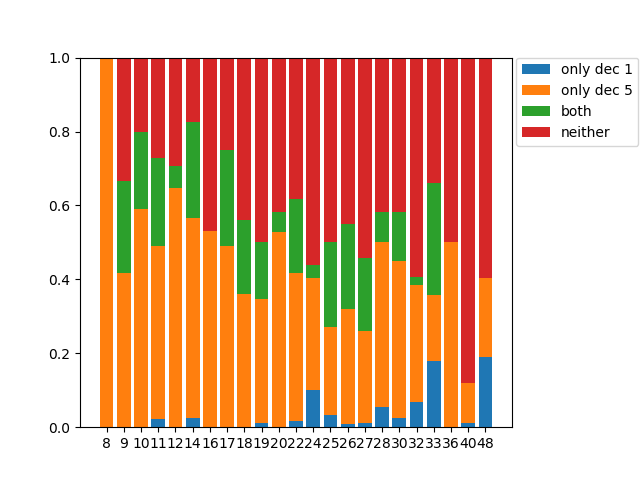
\includegraphics[width=.4\textwidth,keepaspectratio]{figures/jump_subset_out.png}
% %    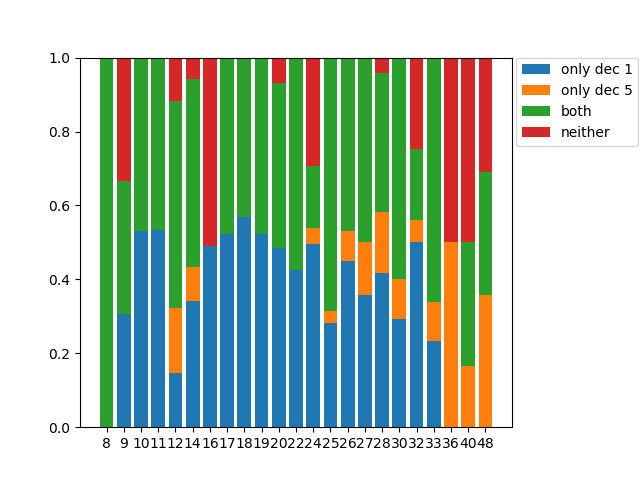
\includegraphics[width=.4\textwidth,keepaspectratio]{figures/template_subset_out.png}
%     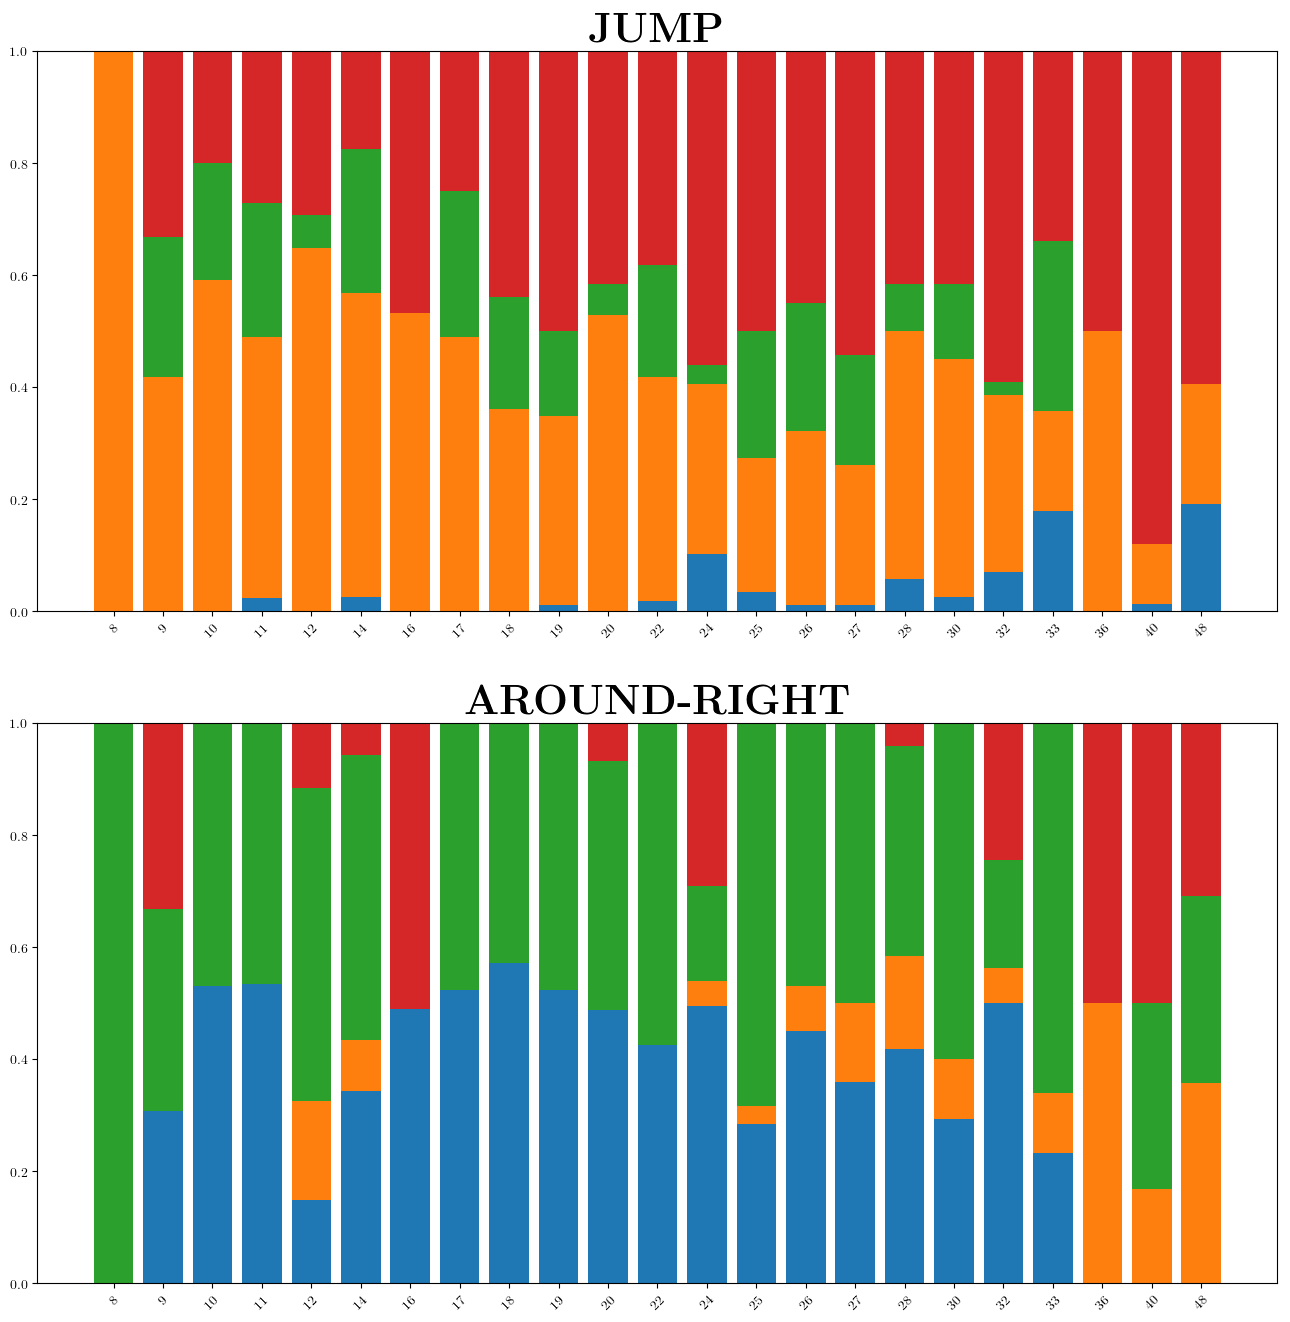
\includegraphics[width=.5\textwidth,keepaspectratio]{figures/split_subset_out.png}
%     \caption{Proportion of items that were correctly executed by
%       models with 5- and 1-decoder widths, in function of ground-truth
%       output length.}
%     \label{fig:kernel_width}
% \end{figure}

\paragraph{Impact of multi-layer attention}
\label{subsec:exp3}

The fairseq CNN features attention from all layers of the
decoder. Is the possibility to focus on different aspects of the input
while decoding from different layers crucial to the better
generalization skills of the CNN? Fig.~\ref{fig:exp3} reports model
accuracy when using attention only from a subset of the 6
layers. Whereas for the \emph{random} split differences are minimal,
ablating attentions greatly affects the performance on the
compositional splits (although in both cases there is a single ablated
configuration that is as good as the full setup).

\begin{figure}[tb]
    \centering
    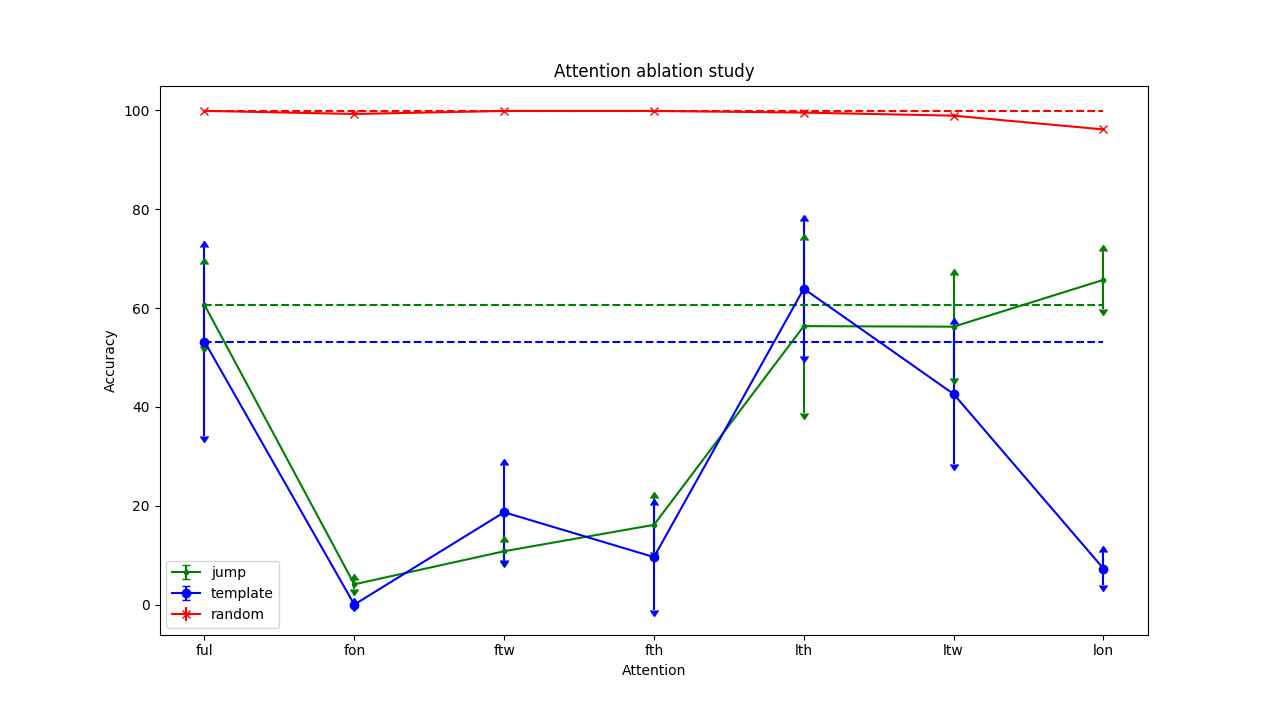
\includegraphics[width=.5\textwidth,keepaspectratio]{figures/attention_exp.png}
    \caption{Accuracy of overall-best model when keeping attention
      only on first layer (\emph{bottom1}), first two layers
      (\emph{bottom2}), \ldots, last two layers (\emph{top2})), top
      layer only (\emph{top1}). Means and standard deviations across 5
      seeds. Dashed lines show full-multi-layer attention results.}
    \label{fig:exp3}
\end{figure}

